%JACS TEMPLATE STARTS HERE
\documentclass[journal=nanofd,manuscript=suppinfo]{achemso}
\usepackage[version=3]{mhchem} % Formula subscripts using \ce{}
\usepackage{lineno,xcolor}
\newcommand*{\mycommand}[1]{\texttt{\emph{#1}}}

%\documentclass[aip,graphicx]{revtex4-1}
%\documentclass[aip,apl,amsmath,amssymb,linenumbers,reprint]{revtex4-1}
%\documentclass[aip,apl,amsmath,amssymb,linenumbers,preprint]{revtex4-1}
\usepackage{graphicx}
\usepackage[version=3]{mhchem} % Formula subscripts using \ce{}
\usepackage{subfig}
\usepackage{dcolumn}% Align table columns on decimal point

\usepackage{amsmath}% amsmath...
\usepackage{bm}% bold math

\usepackage{siunitx}% JMF addition - once a physicist, always a physicist
\usepackage{booktabs}% JMF addition - professional tables; no vertical lines

%\bibliographystyle{aipnum4-1}
%\draft % marks overfull lines with a black rule on the right

\title{PCBM-CG: A place for tired \LaTeX to rest}

\author{Jarvist M. Frost}
\email{j.m.frost@bath.ac.uk}
%\author{Federico Brivio}
%\author{Christopher H. Hendon}
\affiliation{Centre for Sustainable Chemical Technologies and Department of Chemistry, University of Bath, Claverton Down, Bath BA2 7AY, UK}

%\author{Mark van Schilfgaarde}
%\affiliation{Department of Physics, Kings College London, London WC2R 2LS, UK}

%\author{Aron Walsh}
%\email{a.walsh@bath.ac.uk}
%\affiliation{Centre for Sustainable Chemical Technologies and Department of Chemistry, University of Bath, Claverton Down, Bath BA2 7AY, UK}

\begin{document}

\begin{abstract}
Abstract. EPSRC gave us some money so we did our best to do great science, and these are our conclusions. 
\end{abstract}

%\pacs{88.40.-j, 71.20.Nr, 72.40.+w, 61.66.Fn}
% 71.20.Nr 	Semiconductor compounds 
% 72.40.+w 	Photoconduction and photovoltaic effects
% 61.66.Fn 	Inorganic compounds 
% 88.40.jn 	Thin film Cu-based I-III-VI2 solar cells
% 88.40.-j 	Solar energy

%\maketitle 

\textbf{Lambdas}

\begin{table}
\centering
\begin{tabular}{lSSS}
\toprule
Isomer & $\lambda_{neut}$ & $\lambda_{ion}$ & $\lambda_{tot}$ \\
\midrule
mono & 77.91 & 77.49 & 155.40 \\
\midrule
bis-C1 & 111.52 & 182.64 & 294.16 \\
bis-C2 & 108.54 & 158.89 & 267.43 \\
bis-C3 & 81.38 & 83.31 & 164.69 \\
bis-E1 & 88.82 & 89.49 & 178.31 \\
bis-T1 & 138.30 & 151.32 & 289.62 \\
bis-T2 & 80.30 & 80.93 & 161.23 \\
bis-T3 & 125.77 & 166.20 & 291.97 \\
bis-T4 & 87.66 & 95.56 & 183.22 \\
\midrule
tris-E,E,E & 108.42 & 105.41 & 213.84 \\
tris-E,E,T1(1) & 99.51 & 100.82 & 200.33 \\
tris-E,E,T1(2) & 94.62 & 98.86 & 193.49 \\
tris-E,T3,T2 & 93.97 & 92.93 & 186.90 \\
tris-E,T4,T2 & 98.54 & 106.46 & 205.00 \\
tris-E,T4,T3 & 100.51 & 100.06 & 200.56 \\
tris-T3,T3,T3 & 137.97 & 173.63 & 311.60 \\
tris-T4,T3,T3 & 200.30 & 226.34 & 426.64 \\
tris-T4,T4,T2 & 149.22 & 148.26 & 297.48 \\
%tris- & {DATA} & {HERE} & {PLEASE} \\
tris-T4,T4,T4 & 136.01 & 166.56 & 302.57 \\
\bottomrule
\end{tabular}
\caption{\label{tab:Lambda}
Inner sphere reorganisation energies of Mono, Bis and Tris PC$-{60}$BM fullerenes. All units meV.}
\end{table}

\begin{table}
\centering
\begin{tabular}{lSSS}
\toprule
Isomer & $\lambda_{neut}$ & $\lambda_{ion}$ & $\lambda_{tot}$ \\
\midrule
mono & 68.80 & 68.83 & 137.63 \\
\midrule
bis-c1 & 70.42 & 70.57 & 140.99 \\
bis-c2 & 70.45 & 73.48 & 143.93 \\
bis-c3 & 78.69 & 72.39 & 151.08 \\
bis-e1 & 69.79 & 74.79 & 144.58 \\
bis-t1 & 69.37 & 69.01 & 138.38 \\
bis-t2 & 78.85 & 79.53 & 158.38 \\
bis-t3 & 75.42 & 72.98 & 148.40 \\
bis-t4 & 70.03 & 68.63 & 138.66 \\
\midrule
tris-EEE & 105.49 & 78.63 & 184.12 \\
tris-EET1-1 & 76.11 & 76.12 & 152.22 \\
tris-EET1-2 & 72.66 & 72.96 & 145.62 \\
tris-ET3T2 & 73.33 & 75.39 & 148.72 \\
tris-ET4T2 & 75.29 & 72.51 & 147.80 \\
tris-ET4T3 & 76.80 & 73.70 & 150.50 \\
tris-T3T3T3 & 82.08 & 75.01 & 157.09 \\
tris-T4T3T3 & 77.78 & 78.22 & 155.99 \\
tris-T4T4T2 & 74.82 & 74.58 & 149.40 \\
tris-T4T4T4 & 82.84 & 75.88 & 158.73 \\
\midrule
c70-mono & 92.31 & 87.75 & 180.07 \\
c70-bis-4158 & 98.25 & 96.06 & 194.31 \\
c70-bis-5657 & 87.27 & 89.48 & 176.75 \\
c70-bis-6768 & 96.07 & 96.10 & 192.17 \\
\bottomrule
\end{tabular}
\caption{\label{tab:Lambda}
Inner sphere reorganisation energies of Mono, Bis and Tris Methano fullerenes. All units meV.}
\end{table}




\textbf{Some mobs}


\begin{table}
\centering
\sisetup{scientific-notation=fixed,fixed-exponent=-3,round-mode=figures,round-precision=3}
\newcolumntype{H}{>{\lrbox0}c<{\endlrbox}@{}} % Hide some data :^)
\begin{tabular}{lSHSHSH}
\toprule
$\sigma$ & 0.0 & 0.021 & 0.056 & 0.072 & 0.121 & 0.250 \\
\midrule
 M  & 0.004402762    &  0.004071634      &  0.002722337      &  0.002132572      &  0.0008374095     &  4.014195e-05     \\
 B  & 0.002272817    &  0.002067089      &  0.001300517      &  0.0009679719     &  0.0003292884     &  1.183156e-05     \\
 B-E1  & 0.00188074      &  0.00172335   &  0.001089123      &  0.0008162235     &  0.0002771943     &  1.031878e-05     \\
 T  & 0.001201081    &  0.001014771      &  0.0005888677     &  0.000400768      &  0.0001261058     &  3.709921e-06     \\
 T-EEE  & 0.0006229742   &  0.0006152113     &  0.0004291373     &  0.0003060389     &  8.536267e-05     &  2.495028e-06 \\
\bottomrule
\end{tabular}
\caption{\label{tab:mobs}
Simulated mobility by Time of Flight (using the \textsc{ToFET} code), with varying energetic disorder. Units are mobility --- \si{cm^2/Vs}, energetic disorder --- \si{\meV}}
\end{table}


\textbf{Coarse grain fullerene adduct molecular dynamics}

Here we extend the Girifalco \cite{Girifalco_PRB_2000} coarse grain buckminsterfullerene (C$_60$) forcefield.
The general principle in the creation of this simple forcefield is in the smearing out of the effective Lennards-Jones interactions of 60 graphitic-like carbons over the surface of a sphere the experimental size of a C60 fullerene.
We believe this to be directly transferable to the interaction of the fullerene cages in functionalised adducts.

Our intent is to simulate the various PCBM adducts with a simple two-bead model for the fullerene cage and the side-chain, modelled entirely with Lennard-Jones interactions for computational efficiency.
This model for the side-chain of a single spherical super-atom is likely to be better for more symmetric sidechains than PCBM such as indene-functionalised fullerenes.

We created an atomistic model for mono-PCBM based on the OPLS \cite{OPLS} empirical force-field, with the reference geometry from a gas-phase quantum chemistry calculation (b3lyp/6-31g*), and the fullerene cage simulated as arbitrarily stiff.
This we used to do molecular dynamics on a small ensemble (TODO: MD params atomistic) to generate radial distribution functions which we used to fit the coarse-grain molecular dynamics model.

In our coarse-grain model, we choose the interaction energy of the sidechain bead to be the same as the Girifalco parameter for the fullerene site, scaled by the mass of the sidechain (190 Da versus 720.6 for C$_{60}$).

We then compared coarse-grain radial distribution functions to the atomistic model, varying the effective bond length of the fullerene-sidechain connection, and the effective van-de-Waals radius of the sidechain.

$ V_{LJ} = 4 \epsilon (\left ( \frac{\sigma}{r} \right )^{12} - \left(\frac{\sigma}{r}\right )^{6}) $

With $\epsilon_{C60}=26.823$ kJ/mol, $\sigma_{C60}=0.895$ nm; $\epsilon_{PBM}=10.0$ kJ/mol, $\sigma_{PBM}=0.704$ nm; the C60-PBM bond being $r=0.64$ nm.

Having fitted a coarse grain model for mono PCBM, we then extended this to the various fullerene isomer adducts by added extra mono-PCBM sidechain sites at the positions of the adducts.

The parameters for the irreducible set of bis and tris isomers were generated by computationally expedient direct enumeration of all possible configurations. Reduction of the set was made with a simple canonical representation (TODO: angles in table for the Supp Info?).

\textbf{Transport simulations on molecular dynamic assemblies}

We approximate the electron transfer integral between fullerenes with an isotropic approximation where $J \propto exp (-\alpha d)$ where $d$ is inter-fullerene cage distance and $\alpha$ is $0.5 \AA^{-1}$.

Our choice of an isotropic transfer integral is due to the simplicity of extracting this single dimension $d$ from the coarse-grain molecular-dynamics simulation, without needing to consider the attitude of individual molecules. Our previous work\cite{kwaitowski_fullerene} shows that the variation in transfer integrals between unfunctionalised fullerenes varies by [TODO: check this] a factor of two, a relatively small effect compared to variations due to packing.

The cyclo-addition of fullerenes to form the functionalised adducts we study in this work profoundly alters the electronic structure of the fullerene (each addition consumes a (pi orbital) conjugated [TODO: not right wording] electron in forming the sidechain bond).
Even different isomers have explicitly different molecular orbital energy levels \cite{Jarvist_AM_2010}.

Here we use an isotopic transfer integral to approximate the full treatment which would require electronic structure calculations of a wide range of different fullerene adduct isomers.
We postulate that the variation in real-world mobilities can be explained through the variation of fullerene-fullerene packing caused by the various sidechains, and by the consideration of the varying isomer energy levels \cite{Jarvist_AM_2010} as a Gaussian distribution imposed on the site-energies in the semi-classical Marcus equation.


Simulations of time of flight transients were carried out using the ToFeT package \cite{ToFeT}.

\textbf{References}

(Girifalco-PRB-2000) PRB,LA Girifalco, Volume 62, Number 19, 15th Nov 2000


\textbf{Sidechain Enumeration}

C60 has 90 bonds between the 60 atoms. 30 of these are 6,6 coordinating (1.37
A long - along two hexagonal facets) and have more double-bond like character.
The remaining 60 bonds are 5,6 coordinating (1.448 A long). PCBM is formed by
4+2 cycloaddition.
These sidechains are believed (ref - that synth paper) to
wholly coordinate with the 6,6 bonds.

The 8 unique bis isomers, and 45 tris isomers, have been identified and their
point group derived in previous work (ref, Hirsch?).
However we did not find a computationally readable list of structures which
would be directly useful in constructing our coarse grained model.

\begin{figure}[ht!]
    \begin{center}
        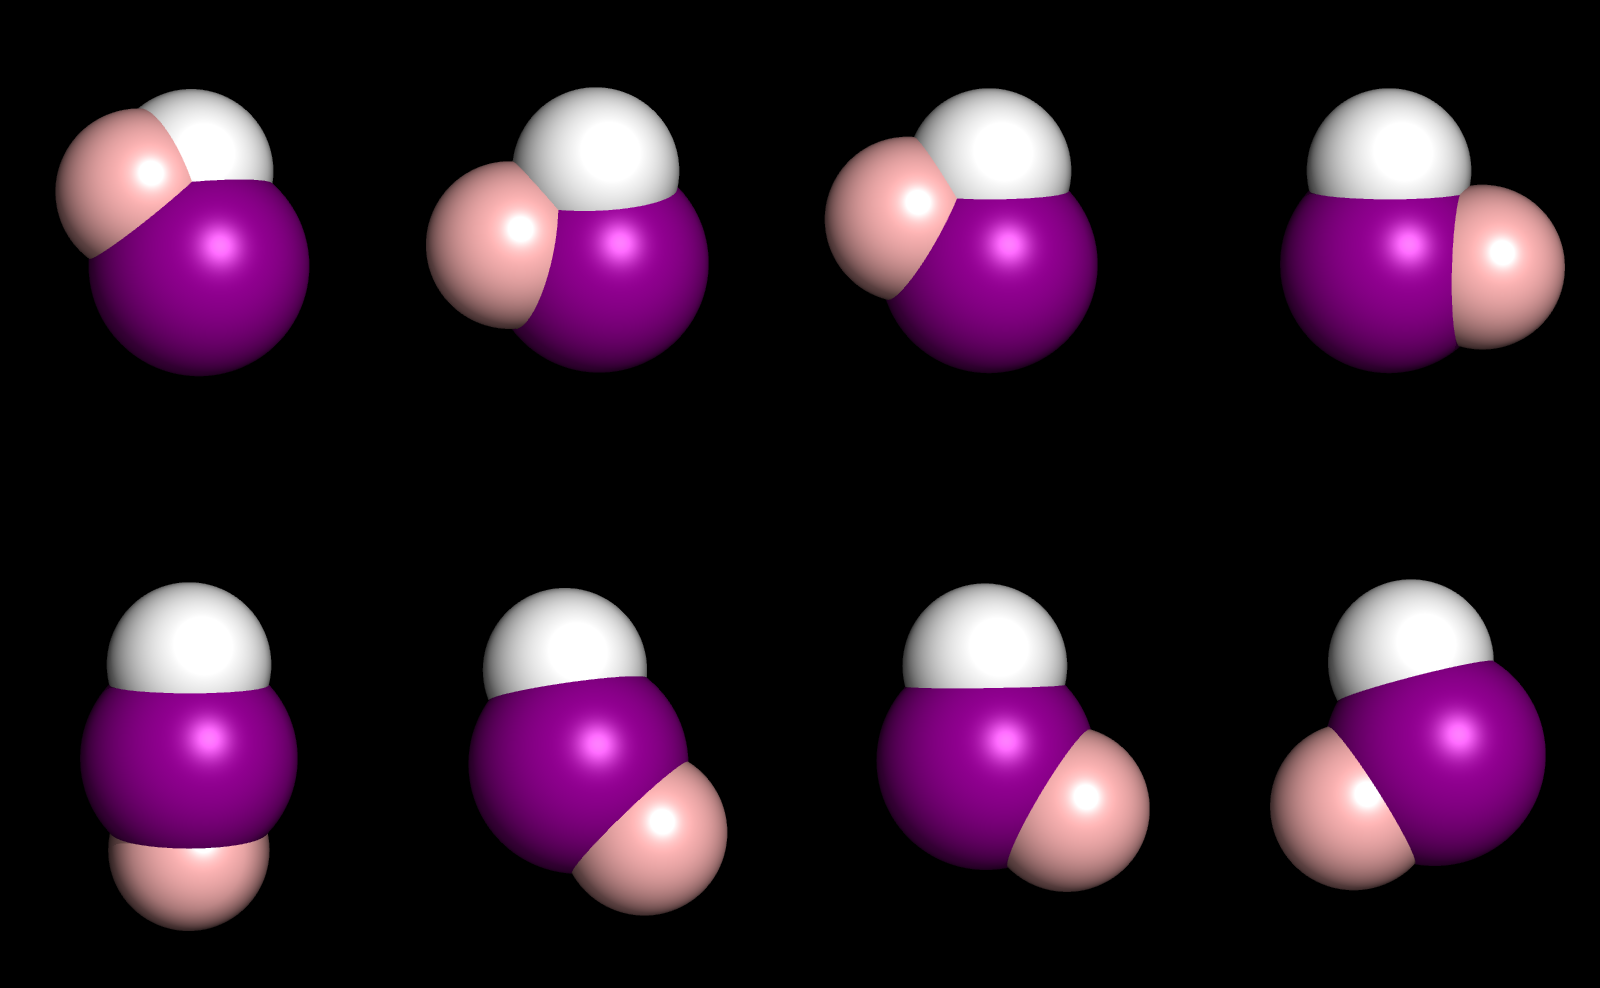
\includegraphics[width=\textwidth]{bis_8_isomers_ray.png}
            \caption{\label{fig-8bisCG}The 8 unique bis isomers, at the coarse grain level.}
    \end{center}
\end{figure}

The bis isomers can be enumerated (identified) by hand and are defined in our
coarse grain model simply as the internal angle between the two sidechains. Of
the 9 unique isomers, two are equitorial, which for our coarse grain model
results in equivalent 90-degree angles.

Identifying unique tris isomers is much more difficult, so we developed
a computational method to directly enumerate the isomers and calculate the
coarse-grain specification of angles between the three sidechains.

First we read in the coorinates of a C60 molecule with (0,0,0) defined as the
centre of the fullerene. We then identify the 6,6 bonds by spacing (<1.4A)
between atoms.
The midpoint of these bonds, and thus the attachment point of the sidechains,
was found by averaging the cartessian positions of the two bonded atoms.

We can then enumerate over all possible permutations of these bonds (30
options, 3 selections leading to 24360 permutations, which can be immediately
simplified by inspection to 812 permutations by taking 2 selections of 29
options if we choose the first location for the first sidechain).
Three inter-sidechain angles are then generated (arcos of the dot production)
from these sets of 3 coordinates (a,b;a,c;b,c).

As the order in which we specify the inter-sidechain angles does not matter, we
are free to rearrange.
By reordering these angles in ascending order, we can identify degenerate
configurations by direct comparison.

The newly calculated set of three angles is compared against a list of uniquely
defined isomers, and either appended to this list if found to be unique, or
discarded and the degeneracy counter of that (already identified) isomer incremented.

\begin{figure}[ht!]
    \begin{center}
        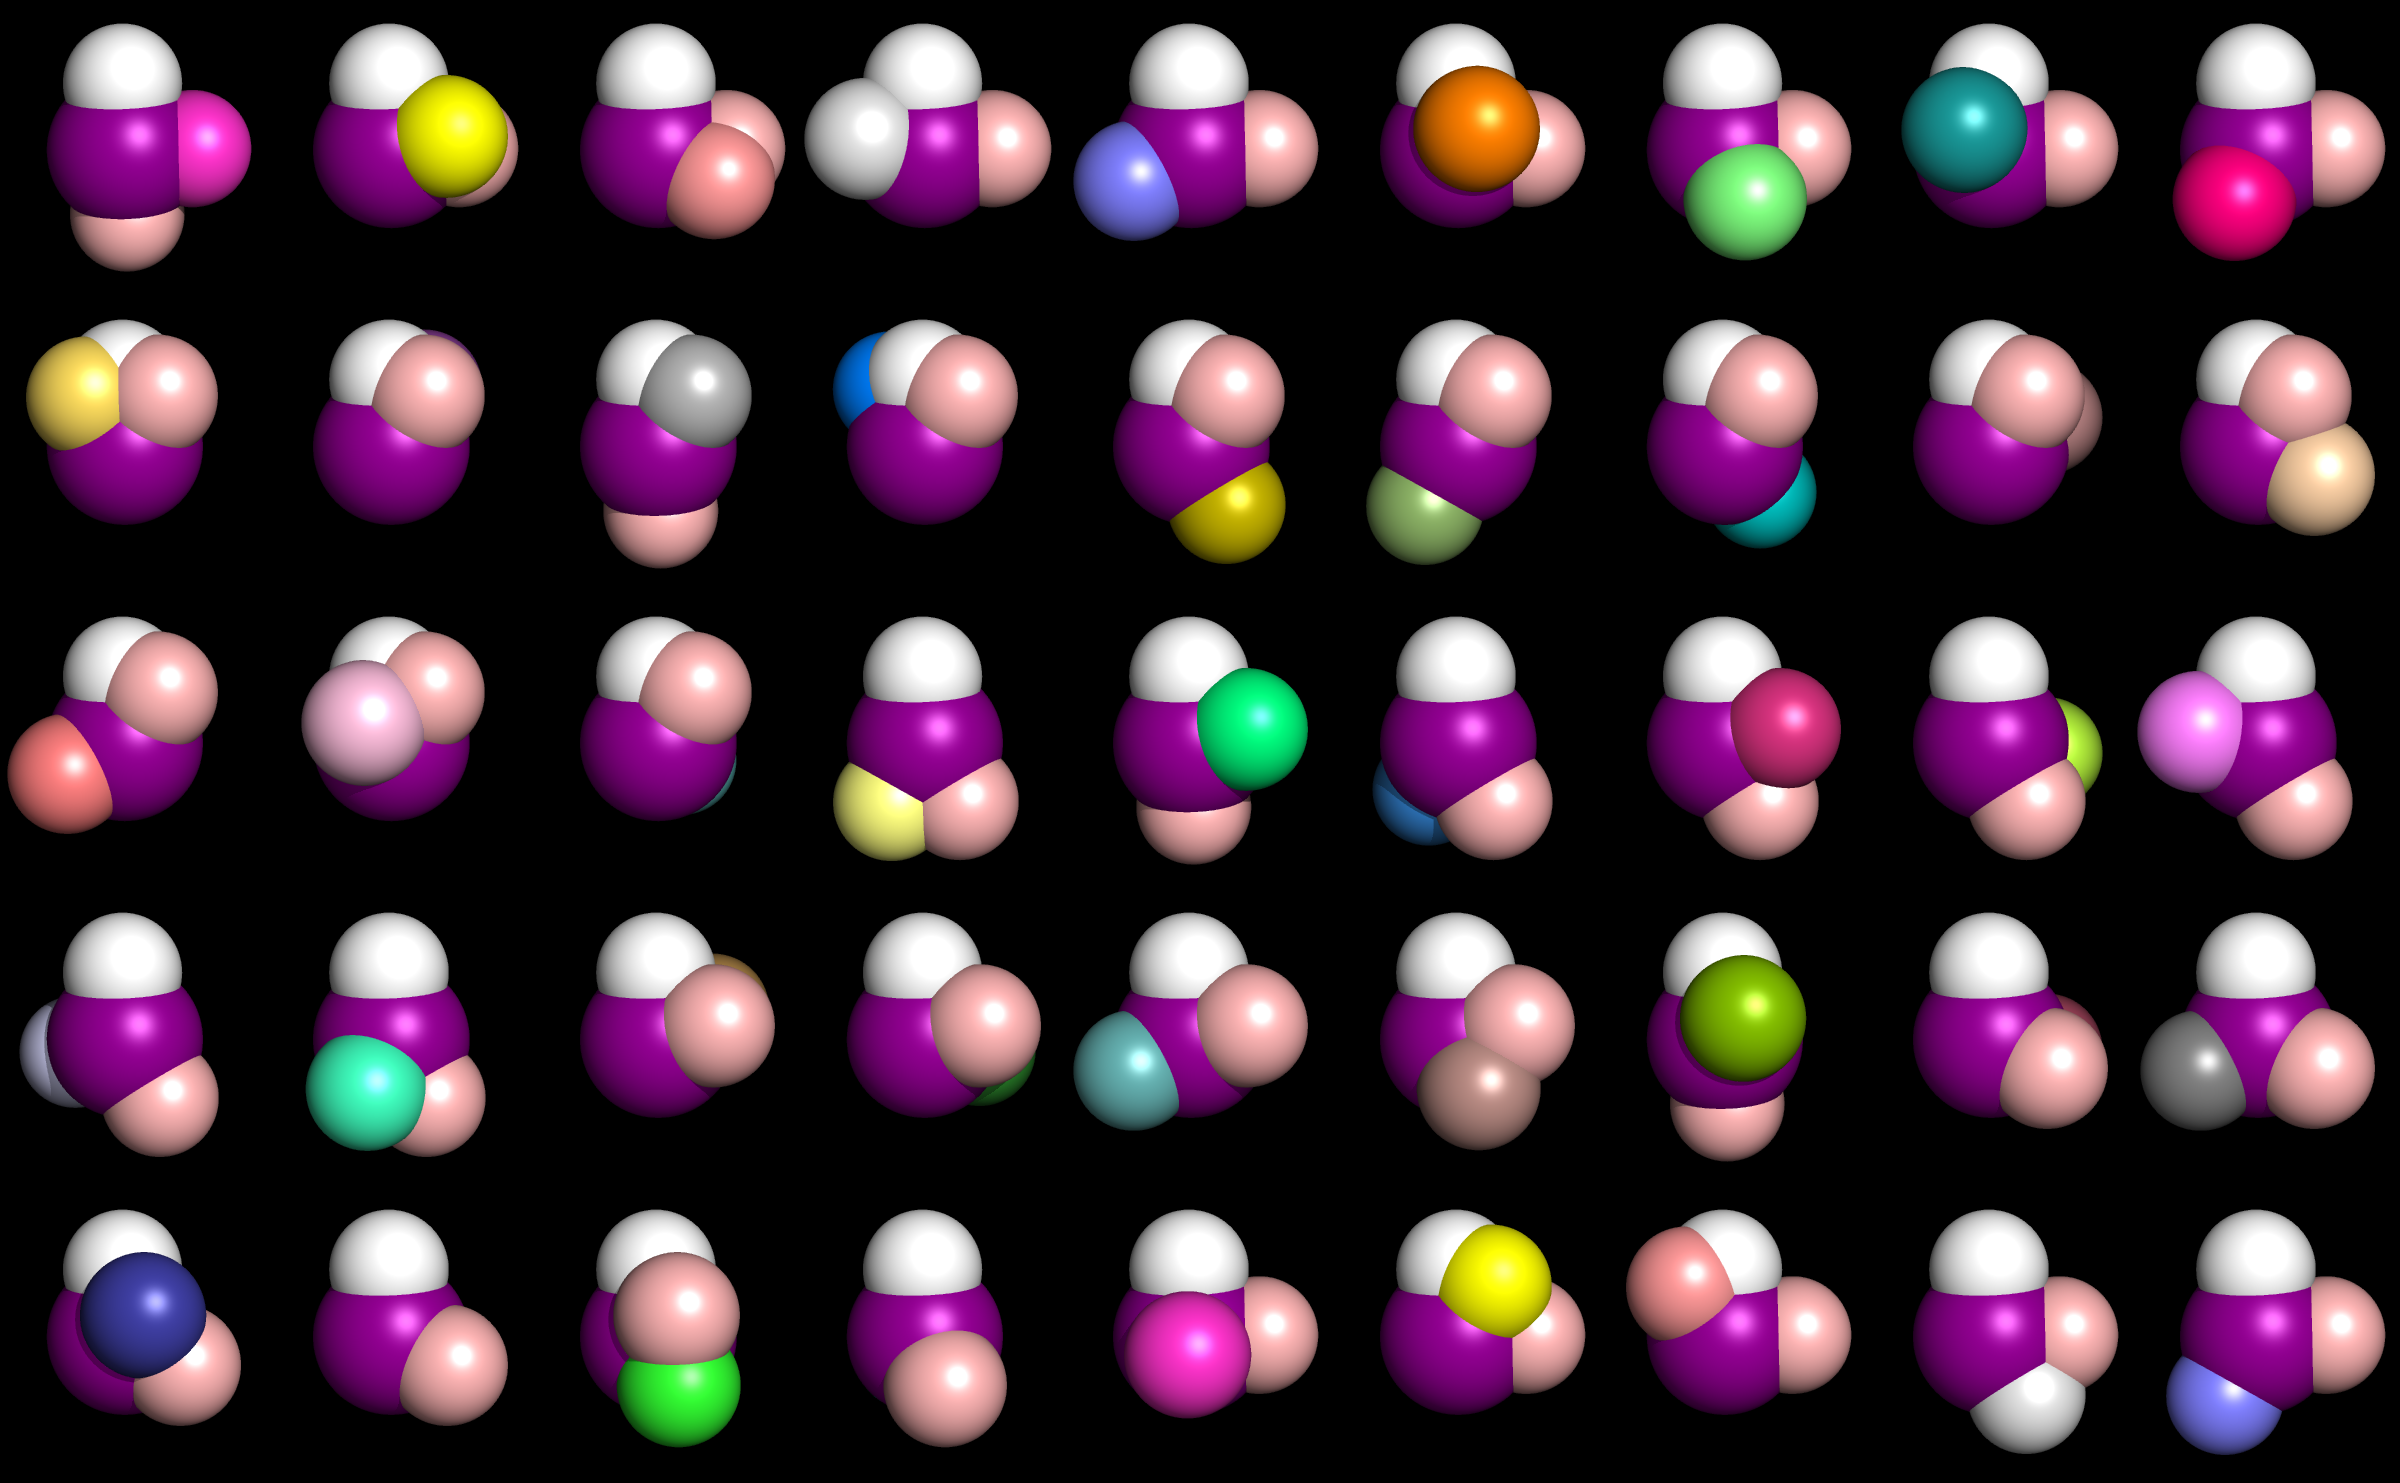
\includegraphics[width=\textwidth]{tris_45_isomers.png}
            \caption{\label{fig-trisCG}The 45 unique tris isomers, at the coarse grain level, as generated automatically by the method described here.}
    \end{center}
\end{figure}

With a simple bit of trigonometry and enumeration we directly discover the 45
unique tris isomers and their symmetry derived degeneracy, and can directly
generate the angle specification suitable for an empirical force field
specificaiton, and a relaxed set of coarse grain coordinates for visualisation
and the generation of a dense initial structure for molecular dynamics.

\begin{table}[ht!]
    \begin{tabular}{lllr}
\toprule
$\theta_{A,B}$ & $\theta_{A,C}$ & $\theta_{B,C}$ & degeneracy \\
\midrule
36 & 36 & 36 & 1 \\
36 & 36 & 60 & 3 \\
36 & 36 & 72 & 3 \\
36 & 60 & 60 & 3 \\
36 & 60 & 72 & 6 \\
36 & 60 & 90 & 6 \\
36 & 72 & 90 & 6 \\
36 & 72 & 108 & 6 \\
36 & 90 & 108 & 6 \\
36 & 90 & 120 & 6 \\
36 & 108 & 120 & 6 \\
36 & 108 & 144 & 6 \\
36 & 120 & 120 & 3 \\
36 & 120 & 144 & 6 \\
36 & 144 & 144 & 3 \\
36 & 144 & 180 & 6 \\
60 & 60 & 108 & 3 \\
60 & 60 & 120 & 3 \\
60 & 72 & 72 & 3 \\
60 & 72 & 90 & 6 \\
60 & 72 & 120 & 6 \\
60 & 90 & 108 & 6 \\
60 & 90 & 144 & 6 \\
60 & 108 & 108 & 3 \\
60 & 108 & 144 & 6 \\
60 & 120 & 144 & 6 \\
60 & 120 & 180 & 6 \\
60 & 144 & 144 & 3 \\
72 & 72 & 108 & 3 \\
72 & 72 & 144 & 3 \\
72 & 90 & 120 & 6 \\
72 & 90 & 144 & 6 \\
72 & 108 & 120 & 6 \\
72 & 108 & 180 & 6 \\
72 & 120 & 144 & 6 \\
72 & 144 & 144 & 3 \\
90 & 90 & 90 & 2 \\
90 & 90 & 180 & 3 \\
90 & 108 & 120 & 6 \\
90 & 108 & 144 & 6 \\
90 & 120 & 144 & 6 \\
108 & 108 & 108 & 1 \\
108 & 108 & 144 & 3 \\
108 & 120 & 120 & 3 \\
120 & 120 & 120 & 1 
\end{tabular}
\caption{\label{table-tris}Inter-sidechain angles for all 45 enumerated tris isomers, with a statement of the degeneracy (number of ways possible of constructing this unique isomer).}
\end{table}

\begin{acknowledgement}
We acknowledge membership of the UK's HPC Materials Chemistry Consortium, which is funded by EPSRC grant EP/F067496. 
J.M.F. is funded by EPSRC Grant EP/K016288/1.
%J.M.F. and K.T.B. are funded by EPSRC Grants EP/K016288/1 and EP/J017361/1, respectively.
%F.B. is funded through the EU DESTINY Network (Grant 316494).
%C.H.H. is funded by ERC (Grant 277757). 
%A.W. acknowledges support from the Royal Society and ERC (Grant 277757). 
We are grateful for the lyrical encouragment of Salt N Pepa. 
\end{acknowledgement}

\begin{suppinfo}
    The data set and analysis codes, \textsc{CoarseGrainPCBM}, are available as a source code and data repository on GitHub\cite{GitHub}.
\end{suppinfo}

\bibliography{library}

\end{document}
